\documentclass{article}

\author{}
\title{Atividade 1 - ES704}

\usepackage[margin=0.8in]{geometry}
\usepackage{indentfirst}
\usepackage{fancyhdr}
\usepackage{tcolorbox}
\usepackage{graphicx}
\usepackage{amsmath}
\usepackage{hyperref}
\usepackage{xcolor}

\hypersetup{
    colorlinks,
    linkcolor={red!50!black},
    citecolor={blue!50!black},
    urlcolor={black!80!black}
}
    

% Create a new command to be used in the align environment in multiple line equations do only the last equation is numbered  
\newcommand{\n}{\nonumber \\ }
\makeatletter
\let\inserttitle\@title
\makeatother
% Set the style of the page 
\pagestyle{fancy}
\fancyhf{}
\rhead{Instrumentação Básica}
\lhead{\inserttitle}
\rfoot{Page \thepage}

% Begin the Document 
\begin{document}

    \maketitle
    \thispagestyle{empty}

    % Add the image inside a figure in as the first page
    \begin{figure}[h]
        \begin{center}
            
\includegraphics[scale = 0.10]{imgs/unicamp.png}
        \end{center}
    \end{figure}

    \begin{table}[b]
        \begin{flushright}
            \begin{tabular}{ll}
                Nome: & Ra: \\ 
                Isabelle Miki Ikuno & 173336\\
                Mateus José de Sousa Goto & 241559\\
                Nuno Kuschnaroff Barbosa & 242616 \\
                Pedro Henrique Limeira da Cruz & 215663
            \end{tabular}
        \end{flushright}
    \end{table}

    % Change to the Next page 
    \newpage

    \section*{Sistema Geral de Medição}
        De forma geral, um sistema de medição possui os seguintes estágios:
        \begin{figure}[h]
            \centering
            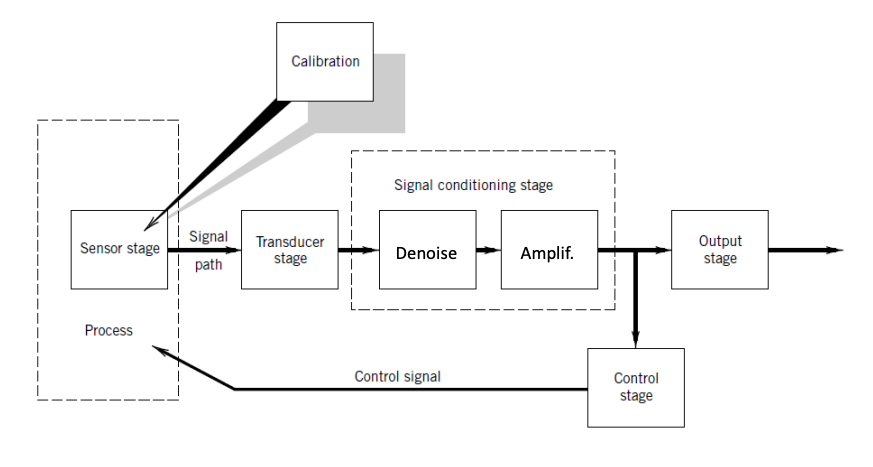
\includegraphics[width=.7\textwidth]{imgs/sis_med_geral.png}
            \caption{Sistema de Medição Genérico}
        \end{figure}

        Quando analisamos o problema em questão, temos que:
        \begin{itemize}
            \item \textbf{Sensor} $\rightarrow$ \textbf{Substrato Piezorresistivo}: Pois o papel do sensor é detectar a mudança em quantidades físicas que, nesse caso, é representado pela deformação e subsequente mudança na resistividade do material.
            
            \item \textbf{Transdutor} $\rightarrow$ \textbf{Ponte de Whetstone}: Pois o papel do transdutor é a conversão de sinais (que no nosso caso converte de resistência para tensão).

            \item \textbf{Calibração} $\rightarrow$ \textbf{processo de calibração estática}: Processo onde aplicam-se excitações de entrada conhecidas e, após a estabilização do sistema, mede-se a saída do sistema. Neste caso, aplica-se forças controladas na matriz tátil a partir de células de carga e então seu sinal é registrado, posteriormente, na saída.
            
            \item \textbf{Signal Conditioning} $\rightarrow$ \textbf{N/A}: Não está necessariamente presente descrito no problema, mas poderia ser utilizado um amplificador de sinais como um \href{https://pdf1.alldatasheet.com/datasheet-pdf/view/1371088/SPARKFUN/HX711.html}{\emph{hx711}}, tendo em vista que a variação de tensão de uma ponte de Whetstone tende a ser pequena.

            \item \textbf{Output Stage} $\rightarrow$ \textbf{Módulo de Aquisição de Sinais}: Tendo em vista que o output stage tem por função armazenar ou indicar o sinal de interesse, após quaisquer tratamentos (se necessários).

            \item \textbf{Controle} $\rightarrow$ \textbf{N/A}: Não especificado.
            
        \end{itemize}

\newpage
\section*{Variáveis}

    As variáveis do sistema podemos ser divididas em: 
    \begin{itemize}
        \item \textbf{Dependente}: Depende de outros fatores/variáveis.
        \item \textbf{Independente}: Independe de quaisquer outras variáveis.
        \item \textbf{Controlada}: Variável a qual seu valor é controlada durante o processo.
        \item \textbf{Não-Controlada}: Variável a qual seu valor \emph{não} é controlada.
        \item \textbf{Externa}: Variável não-controlada, que pode vir a gerar ruído e interferências nas medições.
    \end{itemize}

    Temos, a seguir, uma lista das principais variáveis do processo de medição e suas respectivas classificações.

    \begin{table}[h]
        \centering
        \begin{tabular}{|l|l|c|}
            \hline
            Classificação & Nome & Descrição   \\ \hline

            \textbf{Independente / Controlável} & Força & 
            \begin{minipage}{.4\textwidth}
                \vspace{5px}
                A força que é aplicada sobre o sistema.
                \vspace{5px}
            \end{minipage} \\ \hline
            
             \textbf{Dependente} &
             Deflexão & 
             \begin{minipage}{.40\textwidth} \vspace{5px}
                 Delfexão do substrato e do condutor piezorresistivo 
                 \vspace{5px}
             \end{minipage}\\ \hline

             \textbf{Dependente} & Resistência & 

             \begin{minipage}{.4\textwidth}\vspace{5px}
                 Resistência elétrica do condutor piezorresistivo, dependente da deflexão do substrato.
                 \vspace{5px}
             \end{minipage}\\ \hline
             
            \textbf{Dependente} & Tensão de Saída do Transdutor & 
            \begin{minipage}{.4\textwidth}\vspace{5px}
                Depende da tensão de alimentação, resistência do piezorresistor, por conseguinte, da deflexão e forças aplicadas sobre o substrato.
                \vspace{5px}
            \end{minipage}\\ \hline
            
             \textbf{Externa} & Temperatura & 
             \begin{minipage}{.4\textwidth}
                 \vspace{5px}
                 Temperatura do ambiente, e por conseguinte a temperatura do circuito elétrico, que influencia na resistência elétrica. 
                 \vspace{5px}
             \end{minipage}\\ \hline

             \textbf{Externa} & Alimentação Elétrica & 
             \begin{minipage}{.4\textwidth}
                 \vspace{5px}
                 Influencia as medições de tensão de saída do transdutor (ponto de Whetstone).
                 \vspace{5px}
             \end{minipage}\\ \hline

             
        \end{tabular}
        \caption{Caption}
        \label{tab:my_label}
    \end{table}

\section*{Calibração Estática x Dinâmica}
    A calibração estática aplica uma entrada no sistema e o relaciona, após a extinção do comportamento transiente, a um valor de saída, gerando uma relação direta $y=f(x)$.
    
    Já a calibração Dinâmica aplica uma entrada no sistema e analisa uma resposta transiente, o que possibilita uma resolução temporal, espacial e espectral.

\newpage
\section*{Caracterização do sistema - Curve Fitting}
    Antes de aplicar qualquer método de curve fitting, é necessário identificarmos o comportamento que o sistema possui. Para fazer isso, primeiro realizamos um scatter plot (como visto no primeiro gráfico) para entendermos a tendência dos dados coletados. 
    Verificamos, então, que o sistema possui um comportamento polinomial de segundo grau do tipo $y=p_1x^2+p_2x+p_3$.
    \begin{figure}[h!]
        \centering
        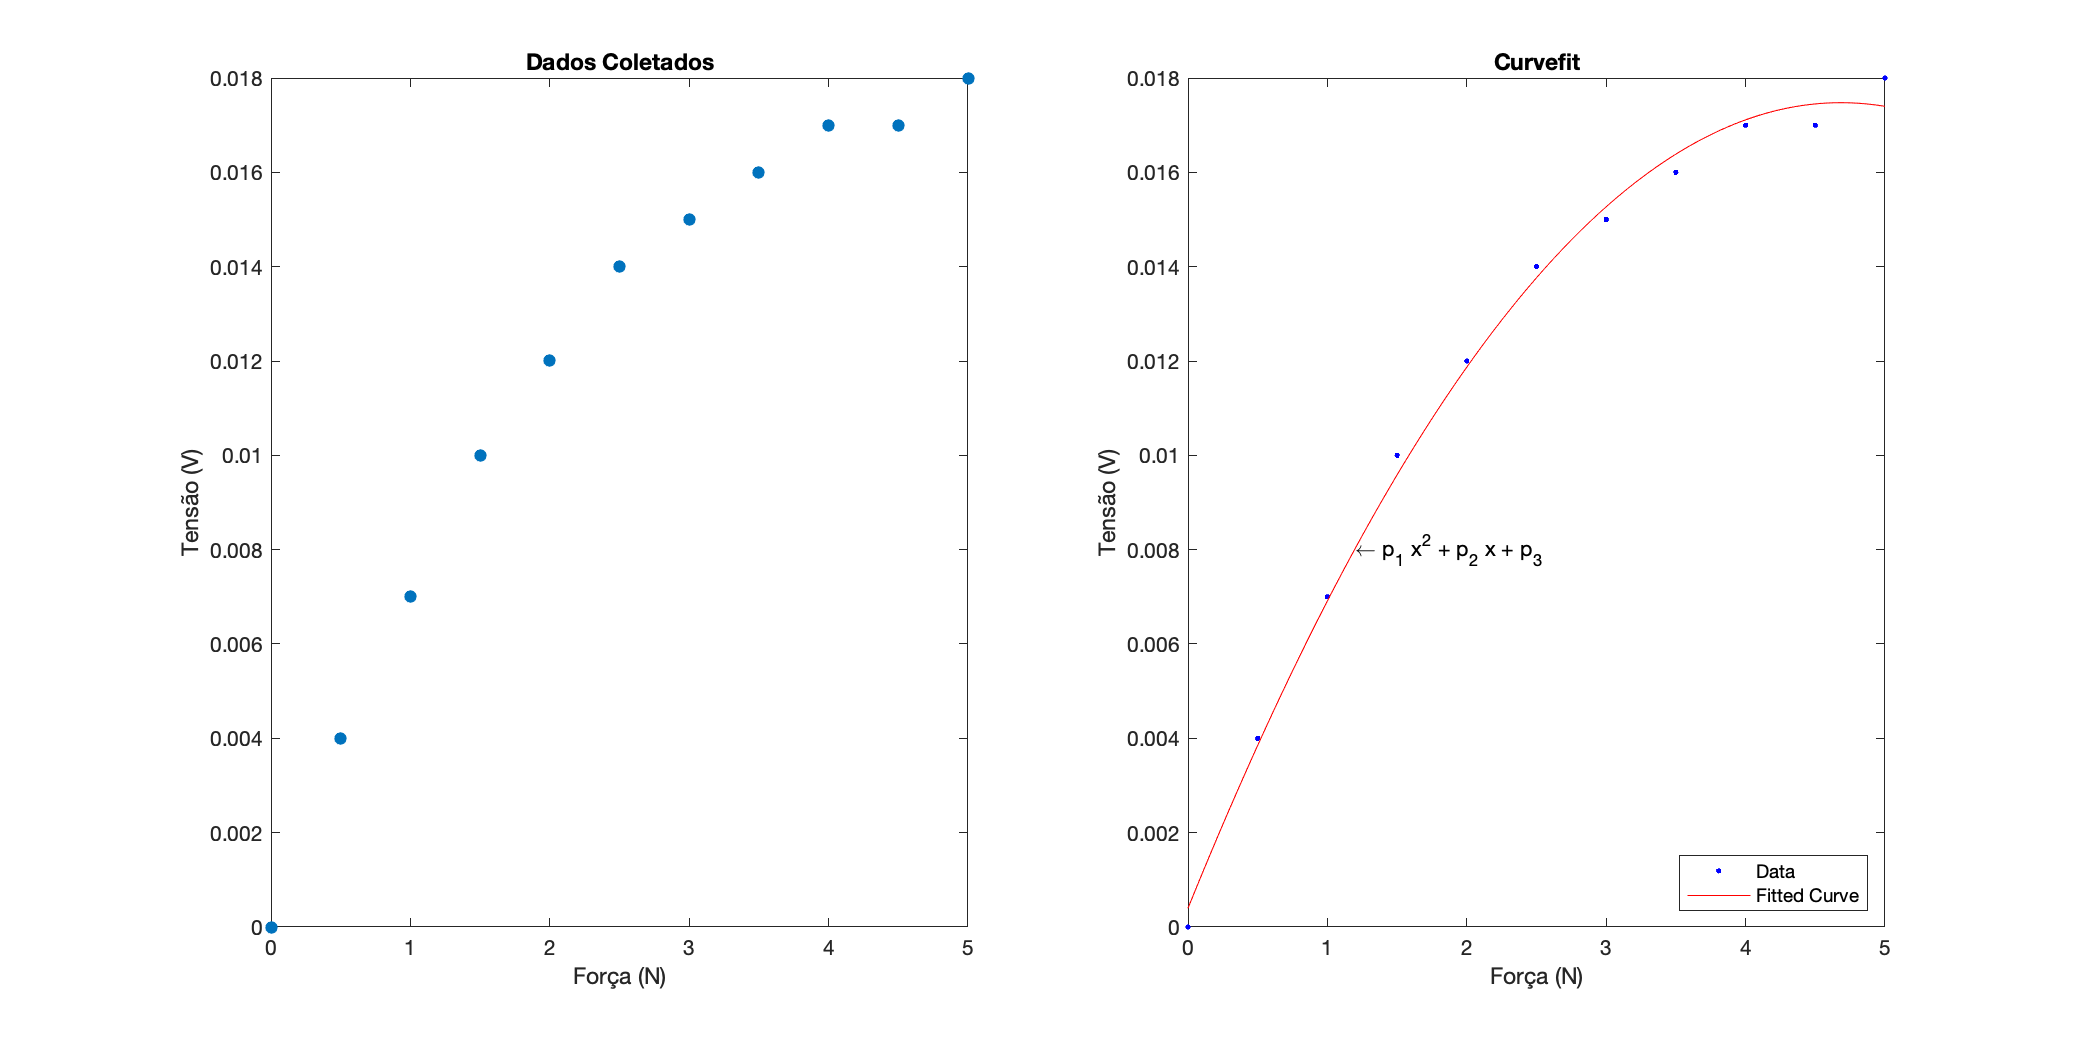
\includegraphics[width=\linewidth]{curve_fitting.png}
        \caption{Curva de Calibração Estática}
        \label{fig:curv_calib}
    \end{figure}

    Após o curve fitting temos, com o coeficiente de determinação $R^2 = 0.95$, os seguintes valores para o polinômio:
    
    \begin{align*}
        \begin{cases}
            p_1 &= -7.786 \times 10^{-4} \\ 
            p_2 &= 7.293 \times 10^{-3} \\
            p_3 &= 3.986 \times 10^{-4}
        \end{cases}
    \end{align*}

    Temos, além disso, as seguintes características da calibração estática feita:
    
    \begin{itemize}
        \item \textbf{Sensibilidade estática}: $\frac{dV}{dF}=-1.557\cdot 10^{-5}x+7.293\cdot 10^{-3}$
        \item \textbf{Faixa dinâmica de entrada}: $0.0\leq F \leq 5.0N$
        \item \textbf{Faixa dinâmica de saída}: $0.000\leq V \leq 0.018V$
    \end{itemize}

\end{document}